\documentclass{article}

\usepackage{lastpage} % for the number of the last page in the document
\usepackage{fancyhdr}
\usepackage{geometry}
\usepackage{graphicx}
\usepackage{grffile}
\usepackage[utf8x]{inputenc}
\geometry{a4paper}
\geometry{portrait}
\pagestyle{fancy}
\usepackage{float}
\fancyhf{}
\lhead{Project Management Information KinderFinder}
\rhead{Section \thesection}
\lfoot{}
\rfoot{Page \thepage\ of \pageref{LastPage}}


%\begin{figure}[H]
%\centering
%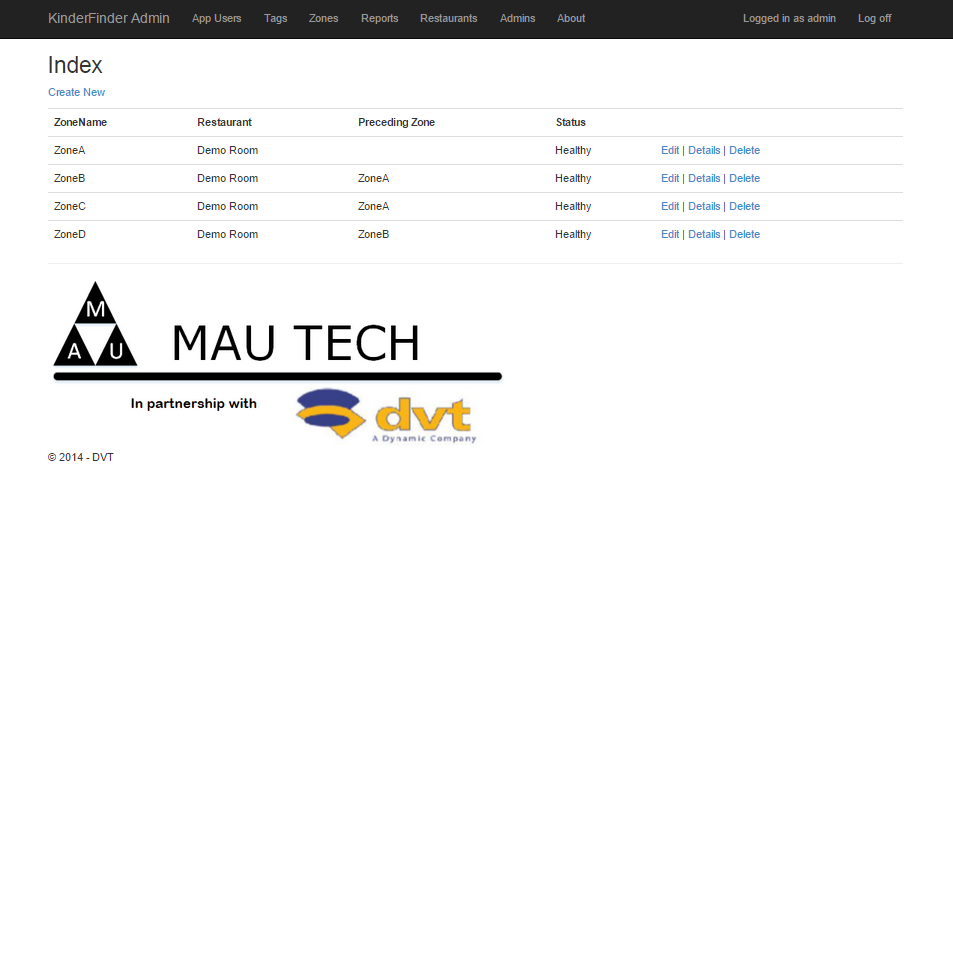
\includegraphics[scale=0.5]{adminportalzones.png}
%\caption{Use case of Android app user (first level granularity).}
%\end{figure}

\newcommand{\horrule}[1]{\rule{\linewidth}{#1}}

\title{
		\normalfont \normalsize \textsc{Client Name: DVT} \\
		\normalfont \normalsize \textsc{Project Name: KinderFinder} \\ [25pt]
		\horrule{0.5pt} \\[0.4cm]
		\huge Project Management Information \\
		\horrule{2pt} \\[0.5cm]
}
\author{\begin{tabular}{rl}
	\texttt{Team Name:} & \texttt{MAU Technologies} \\[0.5cm]
	Uteshlen Nadesan & 28163304 \\
	Michael Johnston & 12053300 \\
	Po-Han Chiu & 11063612
\end{tabular}
	\\ \\ \texttt{}
	\\ \\ \texttt{Version: 1}}
\date{20 October 2014} 


\begin{document}
\maketitle
\newpage

\tableofcontents
\newpage


\section{Software development process}
Our development process employed the Scrum methodology. 

\paragraph{Development Team} The development team consisted of all of us in team MAU Tech.
\paragraph{Scrum Master} Each project undertaken requires a scrum master; Scrum is facilitated by a Scrum Master  who is accountable for removing impediments to the ability of the team to deliver the product goals and deliverables. The Scrum Master is not a traditional team lead or project manager, but acts as a buffer between the team and any distracting influences. Our scrum Master was the Team Leader who made sure the scrum was followed.


\newpage
\section{How Our Software Development Process was Implemented}
\subsection{Sprints}
\paragraph{}
A sprint (or iteration) is the basic unit of development in Scrum. Our Sprints involved iterating through the different use cases we had developed and completing them before moving on to the next use case.
\paragraph{}
Each sprint was started by a planning meeting, where the tasks for the sprint were identified and an estimated commitment for the sprint goal was made, and ended by a sprint review-and-retrospective meeting where the progress is reviewed and lessons for the next sprint were identified.

\subsection{Meetings}
\subsubsection{Sprint planning meetings}
\paragraph{}
At the beginning of the sprint cycle, a Sprint planning meeting was held where we
\begin{itemize}
\item Select what work is to be done
\item Prepared the Sprint Backlog that details the time it will take to do that work, with the entire team
\item Identify and communicate how much of the work is likely to be done during the current sprint
\end{itemize}

\subsubsection{Daily scrum meeting (Almost Daily)}
Each day during the sprint, a project team communication meeting occurred.
\paragraph{}All members of the development team came prepared with the updates for the meeting
\paragraph{}All meetings started precisely on time even if some development team members are missing

\paragraph{}During the meeting, each team member answers three questions
\begin{enumerate}
\item What have you done since yesterday?
\item What are you planning to do today?
\item Any impediments/stumbling blocks?
\end{enumerate}
\paragraph{}Any impediment/stumbling block identified in these meetings were documented by the Scrum Master and worked towards resolution outside of the meeting in the usual sessions we saved for discussion of problem resolution.

\subsubsection{End meetings}
At the end of a sprint cycle, two meetings were held: the Sprint Review Meeting and the Sprint Retrospective meeting.

At the Sprint Review Meeting we
\begin{itemize}
\item Reviewed the work that was completed and the planned work that was not completed
\item Presented the completed work to the stakeholders
\end{itemize}
At the Sprint Retrospective meeting we
\begin{itemize}
\item Reflected on the past sprint
\item Made continuous process improvement
\end{itemize}
This meeting is facilitated by the Scrum Master.

\subsection{Burndown chart}
The sprint burndown chart was publicly displayed where we worked on a white board, it then moved online so we could all see and edit it as need be. It was a chart showing remaining work in the sprint backlog. Updated every day, it gave us a simple view of the sprint progress. It also provided quick visualizations for reference.

\newpage
\section{Profile of Team Members and Responsibilities}
MAU Tech consisted of three members
\begin{itemize}
\item Uteshlen Nadesan
\begin{itemize}
\item Team Leader
\item Scrum master
\item Application Developer
\item Triangulation algorithm
\item Documentation
\end{itemize}
\item Michael K Johnston
\begin{itemize}
\item Vice Team Leader
\item Application Developer
\item Administration Portal Developer
\item Documentation
\item Scrum Board Keeper
\end{itemize}
\item Po-Han Chiu
\begin{itemize}
\item Reporting Developer
\item Application Developer
\end{itemize}
\end{itemize}

\newpage
\section{Plan Used for Issue Management}
We developed a small program that we used as our tracking tool. In this all issues were logged. After the completion of a sprint all issues encountered were checked, and worked on by the entire group with the guidance of our scrum master. 


If there existed an issue we could not fix we were told to contact our client who was always willing to advise us on a way to move forward and a way to fix the issue faced.

\section{Project Status Through Time}
to do
\newpage
\section{List of Functionality You Could Not Implement}
to do
\newpage
\section{Discussion of the Main Risks and Challenges Faced}




\end{document}
